%\documentclass[twocolumn,floatfix,nofootinbib,acs]{revtex4-1}
\documentclass[journal=jpcbfk, layout=traditional, manuscript=article]{achemso}
\setkeys{acs}{articletitle = true}
\usepackage[utf8]{inputenc}


\usepackage{amsmath}    % need for subequations
\usepackage{amssymb}    % for symbols
\usepackage{graphicx}   % need for figures
\usepackage{verbatim}   % useful for program listings
\usepackage{color}      % use if color is used in text
\usepackage{subfigure}  % use for side-by-side figures
\usepackage{hyperref}   % use for hypertext links, including those to external
                        % documents and URLs
\usepackage[capitalise]{cleveref}   % use for referencing figures/equations
\usepackage{soul}
\usepackage{bm}
\usepackage{achemso}
\usepackage{algorithm}
\usepackage{algpseudocode}

\title{Statistical Model Selection for Markov Models of Biomolecular Dynamics}
\author{Christian R. Schwantes}
\affiliation{Department of Chemistry, Stanford University, Stanford CA 94305, USA}
\altaffiliation{Contributed equally to this work}
\author{Robert T. McGibbon}
\affiliation{Department of Chemistry, Stanford University, Stanford CA 94305, USA}
\altaffiliation{Contributed equally to this work}
\author{Vijay S. Pande}
\affiliation{Department of Chemistry, Stanford University, Stanford CA 94305, USA}
\alsoaffiliation{Biophysics Program, Stanford University, Stanford CA 94305, USA}
\alsoaffiliation{Department of Computer Science, Stanford University, Stanford CA 94305, USA}
\alsoaffiliation{Department of Structural Biology, Stanford University, Stanford CA 94305, USA}
\email{pande@stanford.edu}
\keywords{MSM, molecular dynamics, AIC, BIC, Bayes factor}

\mciteErrorOnUnknownfalse

\begin{document}
\maketitle
\begin{abstract}
Markov state models provide a powerful framework for the analysis of biomolecular conformation dynamics in terms of their metastable states and transition rates. These models provide both a quantitative and comprehensible description of the long-timescale dynamics of large molecular dynamics with a Master equation, and have been successfully used to study protein folding, protein conformational change, and protein-ligand binding. However, to achieve satisfactory performance, existing methodologies often require expert intervention when defining the model's discrete state space. While standard model selection methodologies focus on the minimization of systematic bias and disregard statistical error, we show that by consideration of the states' conditional distribution over conformations, both sources of error can be balanced evenhandedly. Application of techniques that consider both systematic bias and statistical error on two 100$\mu s$ molecular dynamics trajectories of the Fip35 WW domain shows agreement with existing techniques based on self-consistency of the model's relaxation timescales, with more suitable results in regimes in which those timescale-based techniques encourage over-fitting. By removing the need for expert tuning, these methods should reduce modeling bias and lower the barriers to entry in Markov state model construction.
\end{abstract}

\section{Introduction}
Proteins are highly complex molecular machines, and their dynamics are an essential aspect of biomolecular function. These dynamics span a wide range of length scales, timescales and complexity, including folding and aggregation, conformational change between functional native sub-states, ligand binding, and allostery \cite{Dobson2003Protein, Kim2008Real, Austin1975Dynamics, Bahar2007Intrinsic}. Whereas classical experimental probes have often been interpreted in two-state frameworks, ensemble measurements with increasingly high temporal resolution as well as sensitive single molecule probes have uncovered a vast array of complex multi-state kinetics \cite{Cosa2006Evidence, Zhang2011Direct}. But the atomic-resolution characterization of these dynamics is often an enormous challenge -- as molecular probes like F\"{o}rster resonance energy transfer, small-angle x-ray scattering, and nuclear magnetic resonance techniques measure complex projections of the intrinsic structure, generally reporting simultaneously on many degrees of freedom\cite{FRET_PAPER?, Mertens2010Structural, Tzeng2011Protein}.

Computer simulations can complement experiments by providing atomic insight into conformational dynamics. With advances at the algorithmic, hardware, and software levels, modern molecular simulation paradigms, incorporating specialized or accelerated hardware, often in combination with highly parallel distributed computing frameworks, are capable of generating extensive simulation ensembles with relative ease\cite{Gotz2012Routine, Eastman2013OpenMM, Shirts2000Screen, Shaw2009Millisecond, Hess2008PLINCS, Buch2010High}. A central challenge in the field of molecular simulations is now often the kinetic analysis, which typically involves constructing a lower resolution model that captures the system's essential features in an interpretable framework\cite{Freddolino2010Challenges, Lane2013Milliseconds}. For example, by projecting the data down onto one or two degrees of freedom we create a simpler model for the system, such as one characterized by diffusion along a single reaction coordinate\cite{Best2010Coordinate}.

Markov state models (MSMs) are one approach for analyzing MD data sets that are able to smoothly move between high and low-resolution models\cite{Chodera2007Automatic, Prinz2011Markov, Beauchamp2012Simple, Bowman2013Quantitative}. High-resolution  models maintain quantitative agreement with the underlying simulation data, while low-resolution models capture the salient features of the potential energy landscape, sacrificing some degree of model complexity. In an MSM, the dynamics are modeled as a memory-less jump process between a discrete set of conformational states which partition the phase space. Two key quantities that define the MSM are thus the state definitions, an indicator function basis over phase space, and the pairwise transition probabilities, which parameterize the kinetics. The matrix of transition probabilities can be used to locate the systems transition paths, and its dominant eigenvectors identify the metastable states and long-timescale dynamical modes\cite{Weinan2006Towards, Deuflhard2000Identification}.

%The trajectory in phase space ($\mathbf{x}_t$) is assigned to one of $k$ states. We represent this assignment by the $s(\cdot)$ function. The dynamics in state space are described by the transition probability matrix. Since the model is Markovian, the probability that a given trajectory in state $s(\mathbf{x}_t)$ will be in some state $i$ is given by $\mathbf{T}_{s(\mathbf{x}_t), i}$:
%\begin{equation}
%\label{eq:markov_state}
%s(\mathbf{x}_{t+\tau}) \sim_d \mathbf{T}_{s(\mathbf{x}_t), i}
%\end{equation} 

%A significant challenge in the automated construction of Markov state models is the choice of the number of states\cite{McGibbon2013Learning}. Although classical Hamiltonian dynamics with $N$ particles form a continuous-time Markov chain in $\mathbb{R}^{6N}$, the projection of this high-dimensional process into a lower dimensional space (such as the discrete indicator functions used by MSMs) is generally governed by non-Markovian dynamics\cite{van1992Stochastic}. \hl{In the Morri-Zwanzig approach, this corresponds to the generalized Langevin equation with a nontrivial memory kernel}(What is this about?)\cite{ZM}. Within the MSM context, on the other hand, this means that first order Markov chains incur a systematic error in their modeling of the high-dimensional system. In particular, when MSM states contain within them kinetic barriers of substantial magnitude, the bias due to the first-order Markov approximation is large. While this source of modeling error can be addressed by increasing the number of states, the reduction in one error comes at the expense of the increase in another. This second source of error is statistical in origin. As the number of states in the model grows, so does the number of parameters required to completely specify the kinetic model between all pairs of states. Because the amount of data is constant, each additional parameter leads to a decrease in the amount of data available per model parameter, which makes the approach susceptible to over-fitting.

Two competing sources of error govern the accuracy of an MSM. The first source of error is systematic and is common to all dimensionality reduction methods. \hl{Any simplified representation of a complex system cannot generally describe arbitrary behavior of that system losslessly.} The second source of error is statistical in nature, in that the parameters of an MSM must be estimated from a finite number of stochastic MD trajectories. \hl{As we discuss later,?} These two sources of error compete in a bias-variance tradeoff\cite{bias_variance_paper}. Given a finite size data set, as the number of states increases, the systematic error (the bias) decreases, while the statistical error (the variance) increases.

Here, we seek to build models that are \emph{suitably} complex, given the data, yielding complex descriptions of the system only to the extent that their additional parameters are implied by the observed dynamics. To that end, we introduce a procedure for scoring the likelihood of an MSM, which, together with standard statistical model selection techniques, enables a balanced selection of the model's parameters. 

\section{Background}
Let $\mathbf{x}_t$ be a ergodic time-homogenous Markov process the phase space $\Omega$ with stationary density $\mu(\mathbf{x})$. Consider an ensemble of such processes at time $t$, described by a distribution $p_t(\mathbf{x})$. There exists an operator, termed the propagator, that evolves the a distribution forward in time at discrete intervals, $\tau$.
\begin{equation}
p_{t+\tau}(\mathbf{x}) = \mathcal{Q}^{(\tau)} \circ p_{t}(\mathbf{x})
\end{equation}
The eigenfunctions of the propagator form a basis for $p(\mathbf{x})$, and the time evolution of the ensemble after $n$ applications of the propagator can be decomposed into a sum of terms along each eigenfunction.
\begin{equation}
\label{eq:prop-timescales}
p_{t+n\tau}(\mathbf{x}) = \sum_{i=1}^\infty \exp\left(-\frac{n \cdot \tau}{t_i}\right) \langle \phi_i, p_t \rangle_{\mu^{-1}} \phi_i(\mathbf{x}),
\end{equation}
where $t_i = -\displaystyle\frac{\tau}{\ln \lambda_i}$ are the propagator's relaxation timescales and $\phi_i$ and $\lambda_i$ are the eigenfunctions and eigenvalues of the propagator, and $\langle \cdot, \cdot \rangle_{\mu^{-1}}$ denotes the inner product defined as
\begin{equation}
\langle \phi_i, p_t \rangle_{\mu^{-1}} = \int_\Omega d\mathbf{x}\; \phi_i(\mathbf{x}) p_t(\mathbf{x}) \frac{1}{\mu(\mathbf{x})}.
\end{equation}
For a more detailed discussion of the propagator and its properties, we refer the reader to \citet{Prinz2011Generation}.

For classical MD, $\mathcal{Q}^{(\tau)}$ is uniquely determined by the Hamiltonian and equations of motion\cite{}. However, it is not practical to explicitly construct the propagator from the Hamiltonian for complex systems. A Markov model provides an estimate for the propagator. A $k$-state Markov model is defined on a discrete set of states, $S = \{s_i\}_{i=1}^k$, where $s_i \subseteq \Omega$ and $\bigcup_{i=1}^k s_i = \Omega$. Furthermore, $s_i \cap s_j = \emptyset$ for all $i \neq j$. In words, every point in $\Omega$ is assigned to one (and only one) state in the MSM. Let $\sigma(\mathbf{x})$ be the function that maps a point $\mathbf{x} \in \Omega$ to the index $i$ of the state in $S$ such that $x \in s_i$.

The MSM models the \hl{action?} of the propagator with a Markov jump process on $\{1, \ldots, k\}$. Let $\mathbf{p} \in (\mathbb{R} \cap [0,1])^k$ be a column vector whose entries sum to one. The elements in $\mathbf{p}$ are defined by a coarse-graining of $p(\mathbf{x})$ over $S$, as
\begin{equation}
\label{eq:coarse-grain-p}
p_i = \int_{\mathbf{x} \in s_i} d\mathbf{x}\; p(\mathbf{x}).
\end{equation} 
Consider a probability vector at time $t$ denoted $\mathbf{p}(t)$. The time-evolution of $\mathbf{p}(t)$ is described by
\begin{equation}
\mathbf{p}(t+\tau)^T = \mathbf{p}(t)^T \mathbf{T},
\end{equation}
where $T_{ij}$ is the probability of transiting to state $j$ in time $\tau$ given that the system started in state $i$. With this construction, the eigenvalues and eigenvectors of $\mathbf{T}$ \hl{provide approximations (what about transfer operator?)} for the eigenvalues and eigenfunctions of $\mathcal{Q}$. In a direct analogy with \cref{eq:prop-timescales}, the eigenvalues $\lambda_i$ of $T$ correspond to relaxation timescales of the Markov model
\begin{equation}
\label{eq:msm-timescales}
t_i = -\frac{\tau}{\ln \lambda_i}.
\end{equation}


Let $D$ be a set of molecular dynamics trajectories in $\Omega$. To construct an MSM, both $S$ and $\mathbf{T}$ must be determined from the data. The state-space, $S$, can be constructed by clustering the points in $D$ or via a grid-based discretization of $\Omega$. Given $S$, maximum-likelihood estimators for the $O(k^2)$ transition probabilities $\mathbf{T}$ exist\cite{kyle, frank}.

Using this procedure, it has been shown that MSM estimates of the eigenvalues $\lambda_i$ are systematically underestimated in the limit of infinite data, and that the magnitude of this bias goes to zero as $k\rightarrow \infty$. This fact has inspired the development of variational methods for model selection, which optimize the MSM parameters in order to maximize the eigenvalues \cite{feliks}.

Selecting the size of $S$ is an important step in model construction, however there is not currently a widely-accepted method in use. Heuristic criteria, such as manually selecting $k = n_\textnormal{conformation} / 14$ or clustering $D$ such that each conformation is within a pre-specified distance to its cluster center (e.g. 4.5\AA$\;$ or 1.2\AA $\;$ RMSD) have been previously employed\cite{Lane2012, Bowman2012, Beuchamp}. Selection of $\tau$ based convergence of the relaxation timescales (\cref{eq:msm-timescales}), as suggested by \citet{Swope2004Describing} and others is more well established. The rate of this convergence with respect to $\tau$ at fixed $S$ has also been used as a metric for evaluating a model's state decomposition. \hl{cite someone?}

\section{The Bias-Variance Dilemma}
For MSM methods to be valuable to practitioners, they must operate in limited data regimes. Thus, we seek a method for model selection that is sensitive to both the systematic error discussed above, as well as the statistical error associated with estimating the model's parameters. Whereas model selection based on the variational principle described above would tend to increase the number of states without bound, as the magnitude of the eigenvalue bias decreases with the number of states, practical application of this criteria would cause a catastrophic increase in statistical uncertainty in the model. This tradeoff between low-variance (small $k$) but biased estimators, and high-variance (large $k$) but unbiased estimators is a general feature of problems in statistical learning\cite{}. For example, as we show in appendix A, the uncertainty in the posterior distribution of $\mathbf{T}$ given $S$ and $D$ grows as $O(k)$.

Introduction to MSMs via the propagator theory motivates the view of the parameterization problem as one of \emph{function estimation}. This perspective has a critical disadvantage: the natural error metric -- the difference between the estimated MSM and true propagator is intrinsically uncomputable. The only access to the true propagator is via samples from the Hamiltonian with MD. Therefore, a compelling alternative is to view the problem as one of \emph{prediction}. Since the MSM is a generative model for trajectories in $\Omega$, it is possible to sample ``pseudo-trajectories" directly from the MSM. If the MSM were perfect, these ``pseudo-trajectories" would be indistinguishable from trajectories generated by the true propagator. Thus, the probability assigned by the MSM, to samples from the true propagator is a measure of the MSM's accuracy. This argument is formalized by Bayes' rule, which establishes a proportionality between the probability of a model given data to the probability of the data given the model
\begin{equation}
\label{eq:bayes}
P\Big(\{S, \mathbf{T}\} \;\Big|\; D\Big) = P\Big(D \;\Big|\; \{S, \mathbf{T}\}\Big) \frac{P(\{S, \mathbf{T}\})}{P(D)},
\end{equation}
where $P\Big(\{S, \mathbf{T}\} \;\Big|\; D\Big)$ is the posterior probability of an MSM, $P\Big(D \;\Big|\; \{S, \mathbf{T}\}\Big)$ is the \emph{likelihood} of the data given a model, $P(\{S, \mathbf{T}\})$ is the prior probability of an MSM before observing any data, and $P(D)$ is the probability of the data, a constant.

\section{Likelihood of a Markov State Model}
Bayes' rule provides a foundation for model selection, by establishing the proportionality of the probability of a model given the data to the probability of the data given the model. Without a strong prior, model selection is reduced to the search for the model that maximizes the likelihood of the data. 
With $\{\mathbf{x}_t\}_{t=1}^N$ an observed trajectory of length $N$, the likelihood can be written as:
\begin{equation}
P\big(\{\mathbf{x}_t\}_{t=1}^N\;\big|\; \{S, T\}\big)d\mathbf{x}^N = \prod_{t=1}^{N-1} T_{\sigma(\mathbf{x}_t), \sigma(\mathbf{x}_{t+1})} \cdot \prod_{t=1}^{N} P(\mathbf{x}_t | \sigma(\mathbf{x}_t)) \cdot d\mathbf{x}^N,
\label{eq:like}
\end{equation} 
where $P(\mathbf{x}_t | \sigma(\mathbf{x}_t))$ is the probability of sampling a conformation $\mathbf{x}_t$ given that the process is in the state $\sigma(\mathbf{x}_t)$, referred to as the emission distribution of state $\sigma(\mathbf{x}_t)$. There is some flexibility in the choice of emission distribution, though \cref{eq:like} is valid only when the emission distributions satisfy
\begin{equation}
P(\mathbf{x} | i) = 0 \;\;\;\; \forall \; \mathbf{x} \textnormal{ s.t. } \sigma(\mathbf{x}) \neq i.
\end{equation}
Given the coarse-graining of $p(\mathbf{x})$ in \cref{eq:coarse-grain-p}, the most natural choice emission distributions are normalized indicator functions
\begin{equation}
P(\mathbf{x} \;|\; i) = \frac{1}{V_i} \mathbf{1}_{s_i}(\mathbf{x}).
\end{equation}
An alternative emission distribution was proposed by \citet{Kellogg2012Evaluation} Instead of having support on $\Omega$, this distribution is supported on the training set $\{\mathbf{x}_t\}_{t=1}^N$. It is given by
\begin{equation}
P(\mathbf{x} \;|\; i) = \big| \{ \mathbf{x}_k : \sigma(\mathbf{x}_k) = \sigma(\mathbf{x}) \} \big|^{-1} \sum_{t=1}^N \delta(\mathbf{x}-\mathbf{x}_t),
\end{equation} where $| \cdot |$ denotes the cardinality of a set and $\delta(\cdot)$ is the Dirac delta function. As this is a discriminative model, it is unable to generalize and assign probability to new data. In certain circumstances, this is an undesirable property. For example, protocols that involve fitting and validating models on separate data sets (e.g. cross-validation) are impossible when the statistical model lacks the capacity to describe new data.

\section{Statistical Model Selection}
Likelihood maximization on the training data (i.e. the data used to fit the model) is insufficient for model selection when the number of parameters varies between proposed models, as more complex models generally exhibit higher empirical likelihoods, often at the cost of larger generalization errors due to over-fitting\cite{Liddle2007Information, Hastie01Elements}. Statistical learning theory provides a number of methods to overcome this problem. Conceptually, the most straightforward is a full Bayesian treatment in which all unknown model parameters are represented by probability distributions. The evidence for a $k$-state model is computed by formally integrating \cref{eq:bayes} over the model parameters and the evidence ratio, or Bayes factor\cite{Gelfand94Bayesian}, then provides a rigorous basis of model selection that appropriately punishes overly complex models as they become poorly constrained in parameter space. Unfortunately such approaches are impractical for problems of this size because of the need to integrate over all possible Markov models of a given size.

Instead, we explore three alternative procedures for choosing the number of states in an MSM: cross validation, Schwarz's Bayesian information criterion (BIC)\cite{Schwartz78Estimating} and the Akaike information criterion (AIC)\cite{Akaike1974AIC}. Cross-validation attempts to directly measure the Markov model's generalization error. First, the model is parameterized by building both the state space and transition matrix on a subset of the available molecular dynamics trajectories, then the likelihood is evaluated on the left-out portion. This scheme can be repeated many times with different partitions of the data set. The AIC and BIC are augmented likelihood function approaches that do not require leaving out portions of the available data during fitting, and instead employ asymptotic approximations to the Bayesian evidence to directly penalize models with additional free parameters.
\begin{equation}
\label{eq:bic}
\mathrm{BIC} \equiv -2\cdot \ln L + \left(\ln N \right)\cdot \kappa
\end{equation}
\begin{equation}
\label{eq:aic}
\mathrm{AIC} \equiv -2\cdot \ln L + \left(2\right) \cdot \kappa
\end{equation} where $L$ is the likelihood, $\kappa$ is the number of free parameters, and $N$ is the number of data points, assumed to be independent and identically distributed. Model selection is performed by a minimization of the criterion.

%\section{Prior Work}

%Given a Markov model parameterized at a lag time of $\tau$, we can propagate ensembles of trajectories via the transition probability matrix:
%$$\mathbf{p}_\tau^T = \mathbf{p}_0^T T(\tau)$$ where $\mathbf{p}_t$ is a probability distribution over states at time $t$ and $T(\tau)$ is a matrix with entries corresponding to the probability of transferring from one state to another at a time of $\tau$. As suggested by \citet{Swope2004Describing}, given a Markov model at a lag time of $\tau$, $T(\tau)$, we expect that a different model with a lag time of $n\tau$ should merely be the $n^\textnormal{th}$ power of $T(\tau)$:
%$$\mathbf{p}_{n\tau}^T = \mathbf{p}_0^T T(n\tau) = \mathbf{p}_0^T \left[T(\tau)\right]^n $$ As such, the eigenvalues and eigenvectors of models built at many lag times are related. Specifically, when building multiple models for the same data set, the eigenvectors should be invariant to changing lag time, while the eigenvalues change via the relation:
%$$\lambda(\tau)^n = \lambda(n \tau)$$ The largest, non-unit eigenvalues correspond to the slowest timescales in the data. It's often useful to compute the slowest implied timescales ($t_i$) via the relation:
%$$t_i = - \frac{\tau}{\log \lambda_i} $$ These implied timescales should be invariant with respect to the lag time and therefore provide a useful tool for testing the quality of an MSM. Specifically, many models are built at varying lag times, and one is selected by choosing the model whose timescales have converged.

%After diagonalization of the transition matrix, the relaxation of any initial probability distribution can be described by a superposition of exponential relaxation processes, with a characteristic time given by $-\frac{1}{\ln \lambda_i}$.
%MSM model selection has traditionally been performed by analyzing the self-consistency of the models with respect to changes in the Markov lag time. In practice, while this test has been useful for many \cite{Noe2009Constructing}, it has some flaws. In particular, it is generally observed that most models' timescales do not converge, but steadily increase, making it difficult to judge whether a particular model passes the test and encouraging the use of ever-more states. Additionally, it is difficult to compare models built on two state decompositions, as neither may have convergent timescales. Often, the choice is made to use the model whose timescales better match an experimental observable.

%Other evaluation strategies include a test based on comparison to a second-order Markov model \cite{Park2006Validation}. Additionally, Bayesian methods that involve marginalizing over all possible MSMs have been developed \cite{Bacallado2009Bayesian, *Bacallado2011Bayesian}. However, these methods are often prohibitively expensive on larger data sets. In contrast, \citet{Kellogg2012Evaluation} proposed a tractable method for comparing MSMs built with different state decompositions, based on a likelihood function for an MD trajectory given an MSM, discussed below.

\section{Methods}
\label{sec:methods}

\subsection{Volume Estimation}
The uniform distribution emission model presents a computational challenge: its use requires the calculation of the (hyper)volume of the MSM's states, which, when defined by clustering, are high-dimensional Voronoi cells. While trivial in two or three dimensions, this computational geometry task becomes challenging in high-dimensional settings. The computation of such volumes has occupied significant attention in recent years in the computational geometry literature, especially via randomized algorithms\cite{Kannan97, Simonovits03, Lovasz03}. We opt to approximate the volumes using Monte Carlo integration, which we find tractable for large systems only when the molecular dynamics data set is first projected into a suitable small vector space of up to perhaps ten dimensions.

A further challenge is the description of the states that are at the edge of the MSM -- whose Voronoi cells extend to infinity in at least one direction. In these cases, the Voronoi cells are of unbounded volume. Instead we wish to truncate these states by bounding them by the convex hull of the data set. Because the convex hull of our simulation data sets are computationally inaccessible, we defined the accessible volume of $\Omega$ denoted $A$, to be the set of all points within a distance $R$ within a set of test points $Y$.

\begin{algorithm}
\caption{Monte Carlo Estimation of the State Volumes}
\begin{algorithmic}[1]
\Procedure{MC Volume Estimation}{$\sigma, A, M$}
	\State $\mathbf{c} \gets [0, 0, \ldots, 0]$\Comment{$\mathbf{c}$ is a vector of length $k$}
	\While{$\sum_{i} c_i \leq M$}
		\State $\mathbf{x} \gets $ sample from axis-aligned hyper cube containing $A$
		\If{$\mathbf{x} \in A$}
			\State $c_{\sigma(\mathbf{x})} \gets c_{\sigma(\mathbf{x})} + 1$
		\EndIf
	\EndWhile
	\State $\mathbf{v} \gets \mathbf{c} \cdot(\sum_{i=1}^k c_i)^{-1}$ \Comment{$\mathbf{v}$ contains the relative volumes of each state}
	\State \textbf{return} $\mathbf{v}$
\EndProcedure
\end{algorithmic}
\end{algorithm} \noindent The result of this scheme produces the volumes of each state relative to the volume of $A$. It's important, therefore, to use the same set $A$ when comparing multiple models.
\subsection{Simulation Protocol}

\begin{figure}
\centering
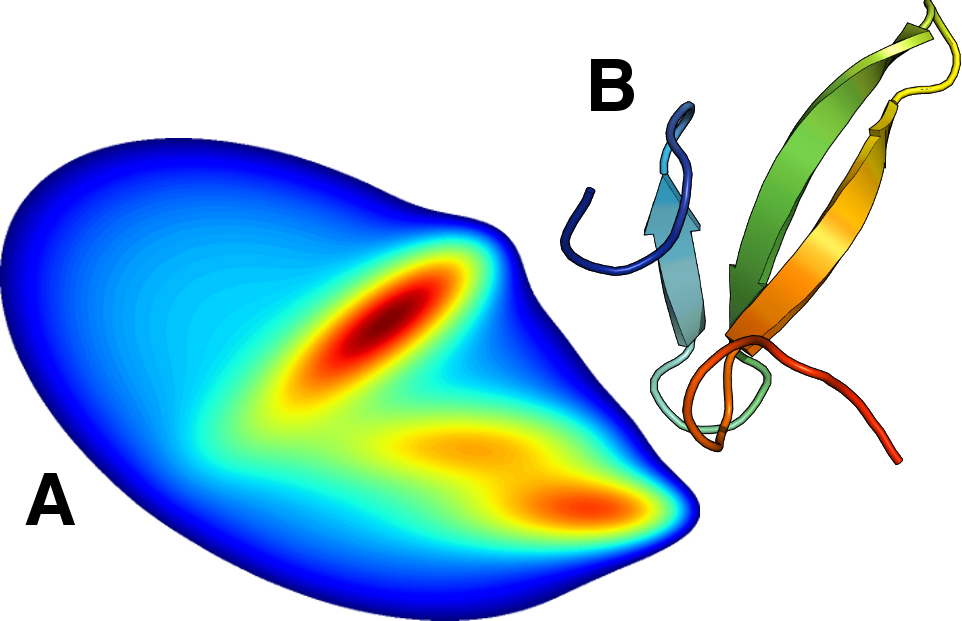
\includegraphics[width=3in]{figs_final/mull_ww.png}
\caption{Systems studied in this work. (A) Brownian dynamics on the two dimensional M\"{u}ller potential \cite{Muller1979Location}. (b) 200 $\mu s$ of dynamics of the Fip35 WW domain\cite{Liu2008Experimental}, courtesy of D.E. Shaw research \cite{Shaw2010Atomic}.}
\label{fig:pics}
\end{figure} 

Two systems were investigated using this likelihood scheme. The first was a simple two dimensional surface with three energy minima, called the M\"{u}ller potential. The dynamics are governed by
$$
\frac{d\mathbf{x}}{dt} = - \nabla V(\mathbf{x})\zeta + \sqrt{2kT\zeta} R(t),
$$ where $\zeta = 10^{-3}$, $kT = 15$, $R(t)$ is a delta-correlated Gaussian process with zero mean, and $V(\mathbf{x})$ was defined as
$$
V(\mathbf{x}) =  \sum_{j=1}^4 A_j \cdot \exp\Big(a_j (x_1-X_j)^2+b_j(x_1-X_j)(x_2-Y_j)+c_j(x_2-Y_j)^2\Big),
$$ where $a = (-1, -1, -6.5, 0.7)$; $b = (0, 0, 11, 0.6)$; $c = (-10, -10, -6.5, 0.7)$; $A = (-200, -100, -170, 15)$; $X = (1, 0, -0.5, -1)$; $Y = (0, 0.5, 1.5, 1)$ as suggested by \citet{Muller1979Location}. Using the Euler-Maruyama method and a time step of $0.1$, we produced two trajectories of length $10^6$ time steps.

The first trajectory was clustered using the $k$-centers clustering algorithm with the Euclidean distance. State volumes were computed for the uniform emission model using $M=10^5$ rounds of Monte Carlo integration defining the set $A$ using the cluster centers from the 50-state model as the test points $Y$ with a cutoff of $R=0.28$. The second trajectory was used as a test set. All MSMs were built using a lag time of 30 steps.

Next, we reanalyzed two ultra-long 100 $\mu s$ molecular dynamics trajectories of the Fip35 WW domain\cite{Liu2008Experimental}, provided courtesy of D.E. Shaw Research \cite{Shaw2010Atomic} (Amber ff99SB-ILDN force field,\cite{amber} TIP3P water model\cite{tip3p}). We projected the trajectories into a four dimensional space using time-structure based independent components analysis (tICA) \cite{Schwantes2013Improvements, Perez2013Identification} on the first trajectory. To calculate the tICs, each conformation was represented as a vector of distances between all pairs of residues separated by at least three amino acids. The distance $d(A, B)$ between residues $A$ and $B$ was determined as follows. Let $\{a_i\}_{i=1}^{n_a}$ and $\{b_i\}_{i=1}^{n_b}$ be the cartesian coordinates of the heavy (non-hydrogen) atoms in $A$ and $B$. Then we define
$$
d(A,B) \equiv \min_{i, j} ||a_i - b_j||_2,
$$ where $|| \cdot ||_2$ denotes the $\ell_2$ norm. The tICs were computed using a correlation lag time of 200 ns. We also performed Principal Components Analysis (PCA) on the same residue-residue distance representation and built MSMs using the top three PCs. In each projection, $k$-centers was used with the Euclidean distance metric.

For the tICA MSMs, the cluster centers from the 100 state model were used as the test points $Y$ to define $A$ with a cutoff of $R=0.81$. In the PCA MSMs, the cluster centers from the 500 state model were used as the test points with a cutoff of $R=2.0$. In each case, $M=10^6$ rounds of Monte Carlo integration were performed to compute the state volumes. All WW MSMs were built using a lag time of 50 ns, which is the same lag time used in previous analyses\cite{Beauchamp2012Simple}.

For both the M\"{u}ller potential and WW models, a maximum likelihood estimator for reversible transition matrices, with a pseudocount of $1 / k$ was used to compute $\mathbf{T}$. The pseudocount ensures that all transitions are assigned nonzero probability, which is especially important for evaluating data that was not used to train the model, as often new transitions will be observed. All analysis and model construction was performed using MSMBuilder \cite{Beauchamp2011Msmbuilder2}.

\section{Results and Discussion}
\subsection{M\"{u}ller Potential}

How well can likelihood-based methods select parameters for an MSM in the data-rich regime? To answer this question, we simulated a simple two-dimensional potential and built a series of MSMs (see ``Methods"). We compared four different model selection criteria: (1) test log-likelihood (2) BIC (3) AIC and (4) implied timescales convergence. The analysis \cref{fig:mullerlike} indicates that the log-likelihood on the training data set continually increases with the addition of further states. The increase is most dramatic at low $k$, and levels off at high $k$, indicating that once $k$ is large enough, the marginal increase in the likelihood with respect to further states is small. For this data set, the log-likelihoods computed on a separate test set exhibit a notably similar trend. Above $k=600$, the test log-likelihood stops increasing. These two trends are to be expected: the additional parameters in the model at higher $k$ never decreases the model's ability to fit the training data. On the other hand, this can lead to the model fitting the statistical noise in the training data set, rather than the system's true dynamics. As result, these "over fit" models at high $k$ are less predictive, as measured by the log-likelihood they assign to new test data.

Leaving out a portion of a molecular dynamics data set from the training to serve as a test set is costly proposition for the applications of MSMs to the study of complex system. For large bimolecular simulations characterized by long intrinsic timescales, sampling the potential exhaustively is a significant challenge\cite{Lane2012}, making it difficult to afford discarding half of the dataset during the fitting of an MSM. For this reason, we also computed two penalized likelihood model selection criteria, the AIC and BIC, which augment the training set log-likelihood with an explicit penalty on model complexity to avoid over fitting. Applied to our simulations of the M\"{u}ller potential, both the AIC and BIC penalize model complexity more strongly than the test set log-likelihood.

The likelihood-based methods are consistent with model selection based on maximization of the implied timescales. For this simple data set, the timescales are maximized by models with 200 states, which agrees with the results obtained with BIC. Model selection based on direct maximization of the implied timescales considers only the systematic error in the MSM, and neglects the statistical error. The consistency between the two approaches on this data set is an indication that the statistical uncertainty is low for these models, which is to be expected given the ease of sampling this two dimensional toy potential.



\begin{figure}[h]
\centering
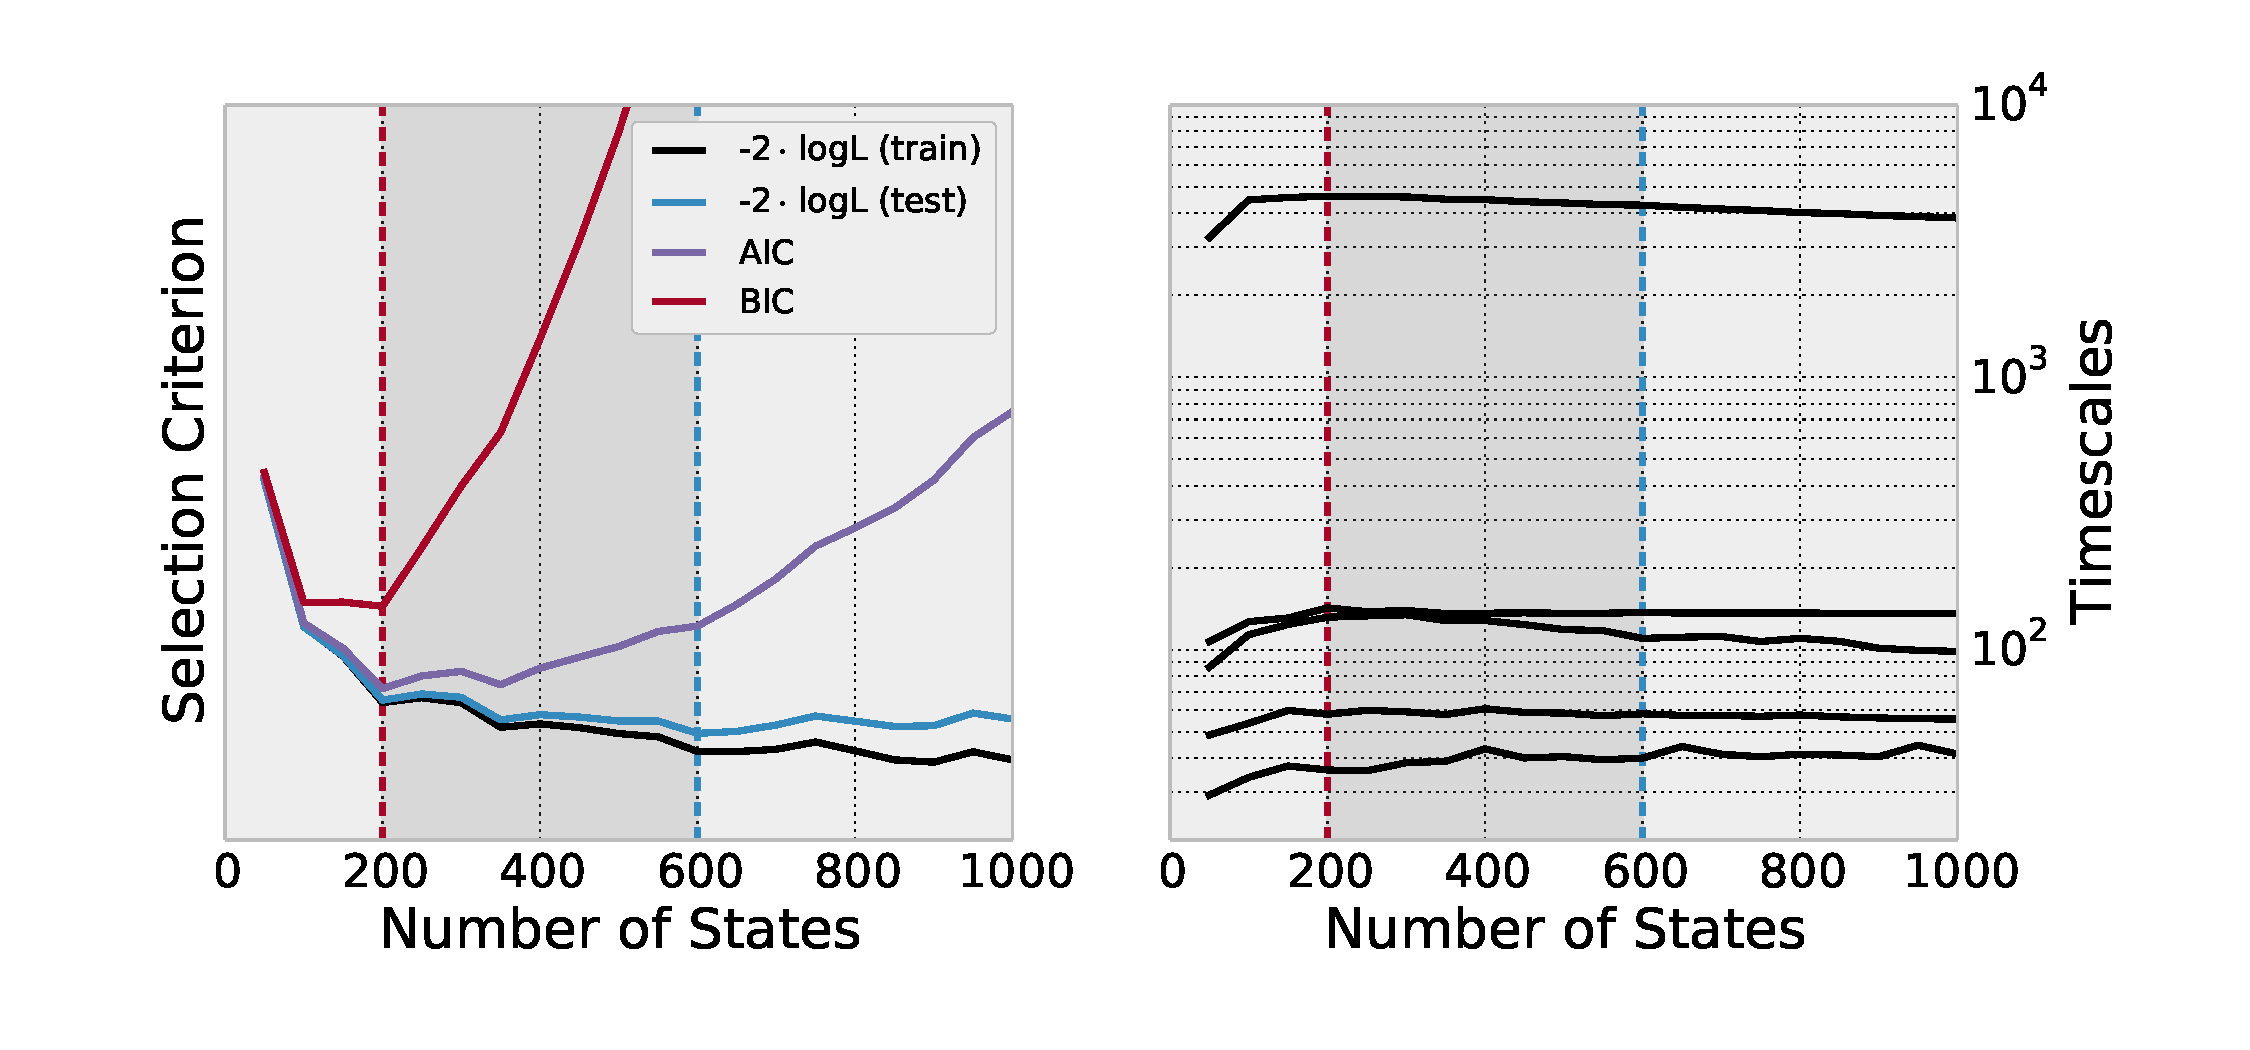
\includegraphics[width=6in]{figs/mull/mull.pdf}
\caption{\hl{Fix this figure so that only part (A) is depicted.} We calculated the training and test set log-likelihoods and model selection criteria for models built with 50-1000 states using the uniform emission distribution. Dashed lines represent the optimal model as defined by the AIC, BIC, or test set log-likelihood and form the boundaries of the optimal window (shaded dark gray). For both likelihoods, the BIC penalizes complexity more than the AIC and test set log-likelihood. The optimal window is consistent with the convergence of the relaxation timescales (right frames).}
\label{fig:mullerlike}
\end{figure}

As shown in \cref{fig:mullerlike}, models built with too few states achieve a drastically reduced likelihood, but above a threshold region the likelihood increases relatively slowly. The penalty on the number of parameters in \cref{eq:bic} and \cref{eq:aic} begins to dominate. The optimal models, according to the BIC, AIC, and test log-likelihood are between 200 and 600 states for this system, which is consistent with the convergence of the relaxation timescales of the models. 

The AIC and BIC penalize the larger state models much more than the test set log-likelihood. It's not clear why the test log-likelihood is more lenient, however, it suggests that when possible, one should use a test log-likelihood approach as opposed to an approximate method like the AIC or BIC. This cross-validation requires fitting multiple models on subsets of the data, and so is not feasible for larger systems in the data-poor regime.

\subsection{Fip35 WW Domain}

Because the likelihood calculations involving the uniform distribution emission model have exponential complexity in the dimensionality of the state space we first preprocess the trajectories with a dimensionality reduction technique.
\begin{figure}
\centering
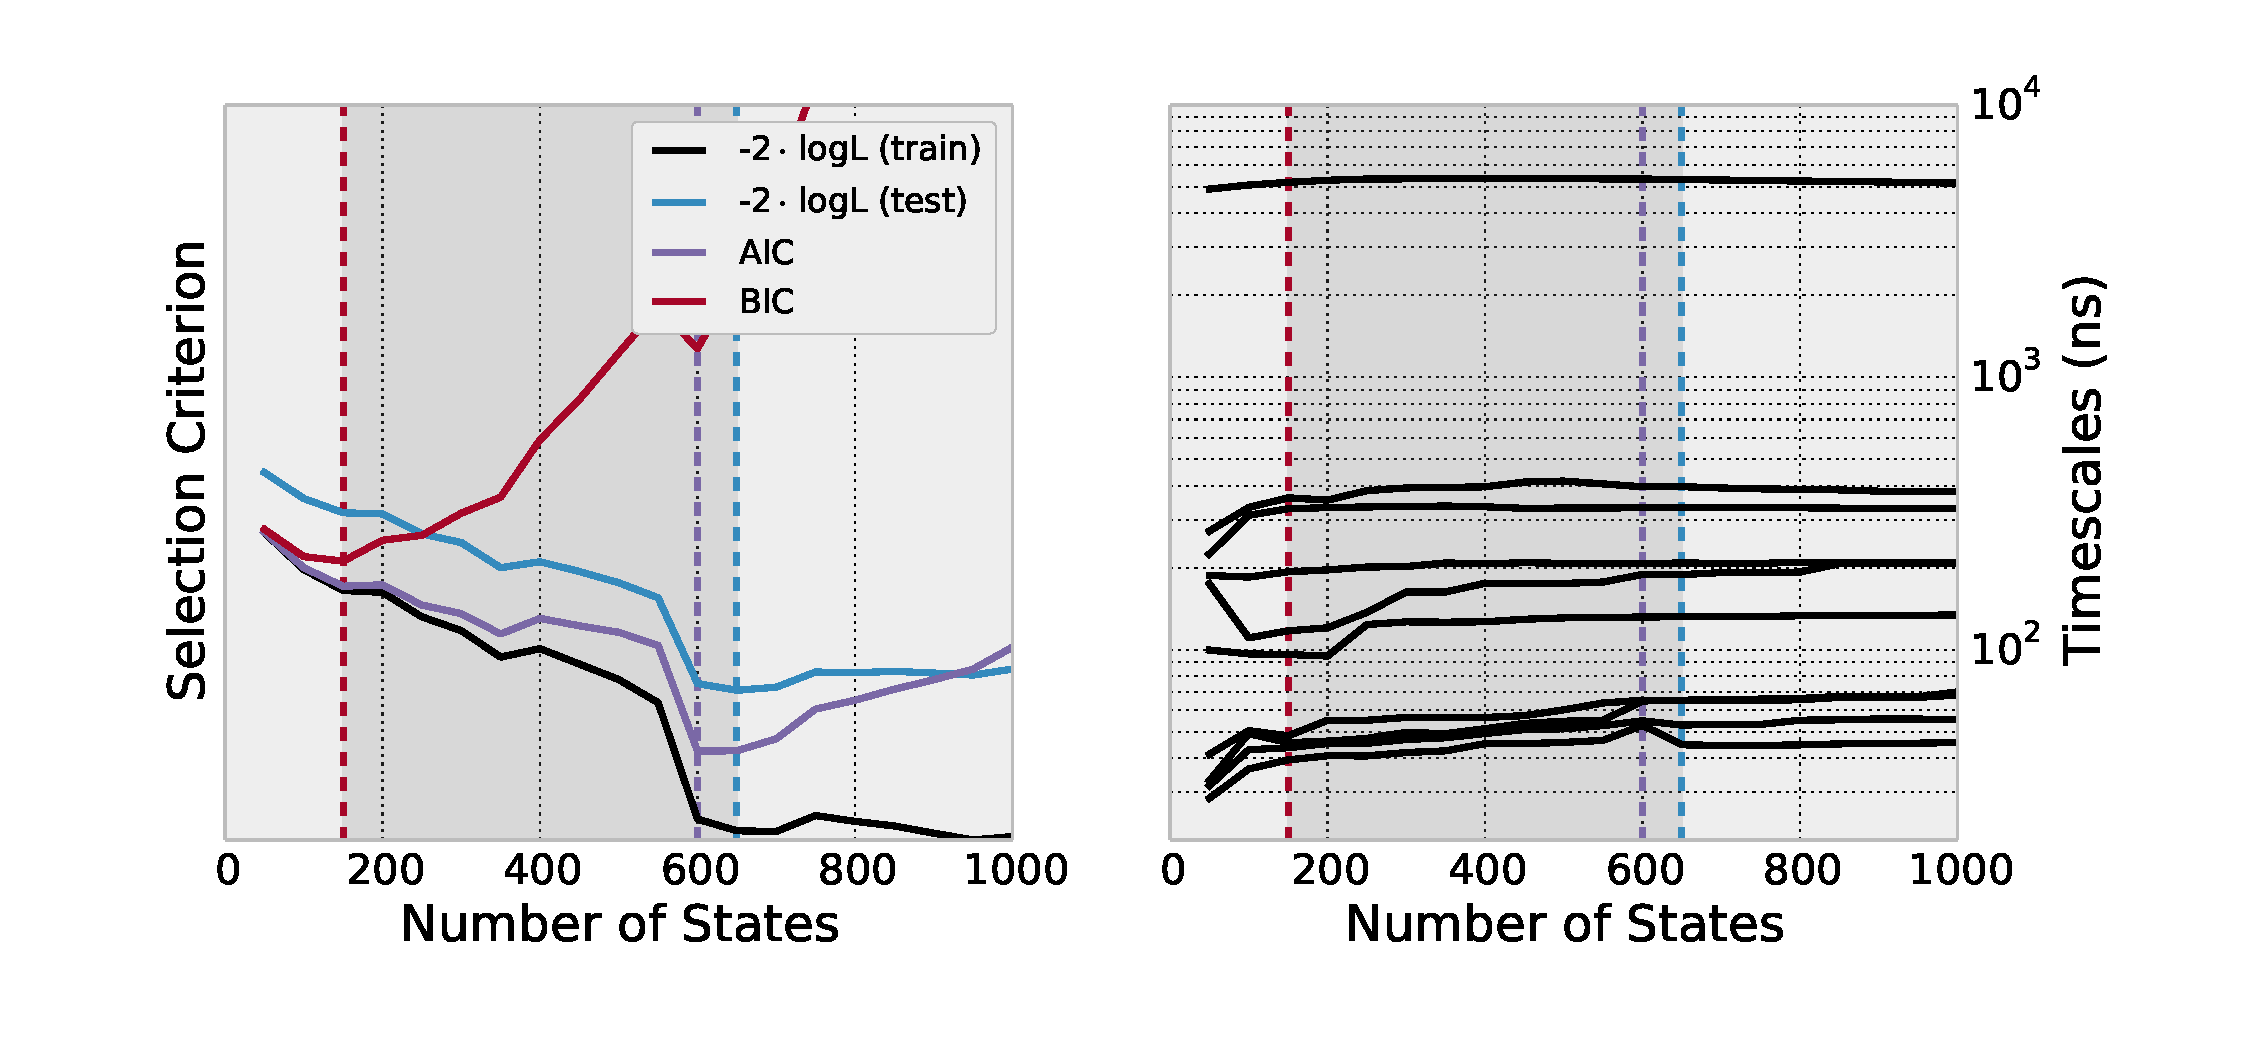
\includegraphics[width=6in]{figs/ww_tica/ww_tica.pdf}
\caption{\hl{Fix this figure so that only part (A) is depicted.} On models whose states were defined after projecting into the four-dimensional tICA subspace, we computed likelihoods based on the uniform emission models. Dashed lines represent the optimal model as defined by the AIC, BIC, or test set log-likelihood and form the boundaries of the optimal window (shaded dark gray). \label{fig:ww}}
\end{figure}

For the models built in the tICA subspace, the AIC is comparable to the test set log-likelihood scores using either emission model, displaying a optimum at ~600 states (\cref{fig:ww}). The BIC penalizes complexity more strongly with an optimum at ~150 states. This window is consistent with the convergence of the relaxation timescales and the onset of Markovian behavior. Models built with RMSD require significantly more states than the tICA MSMs and show poor timescale convergence. These results indicate why model selection based on relaxation timescales is so difficult, as a less than optimal state decomposition can result in timescales that do not converge rapidly (if at all). Furthermore, selection based on only the relaxation timescales contains no guard against over-fitting, which is of particular concern in the models built using RMSD that require thousands of states.

\begin{figure}
\centering
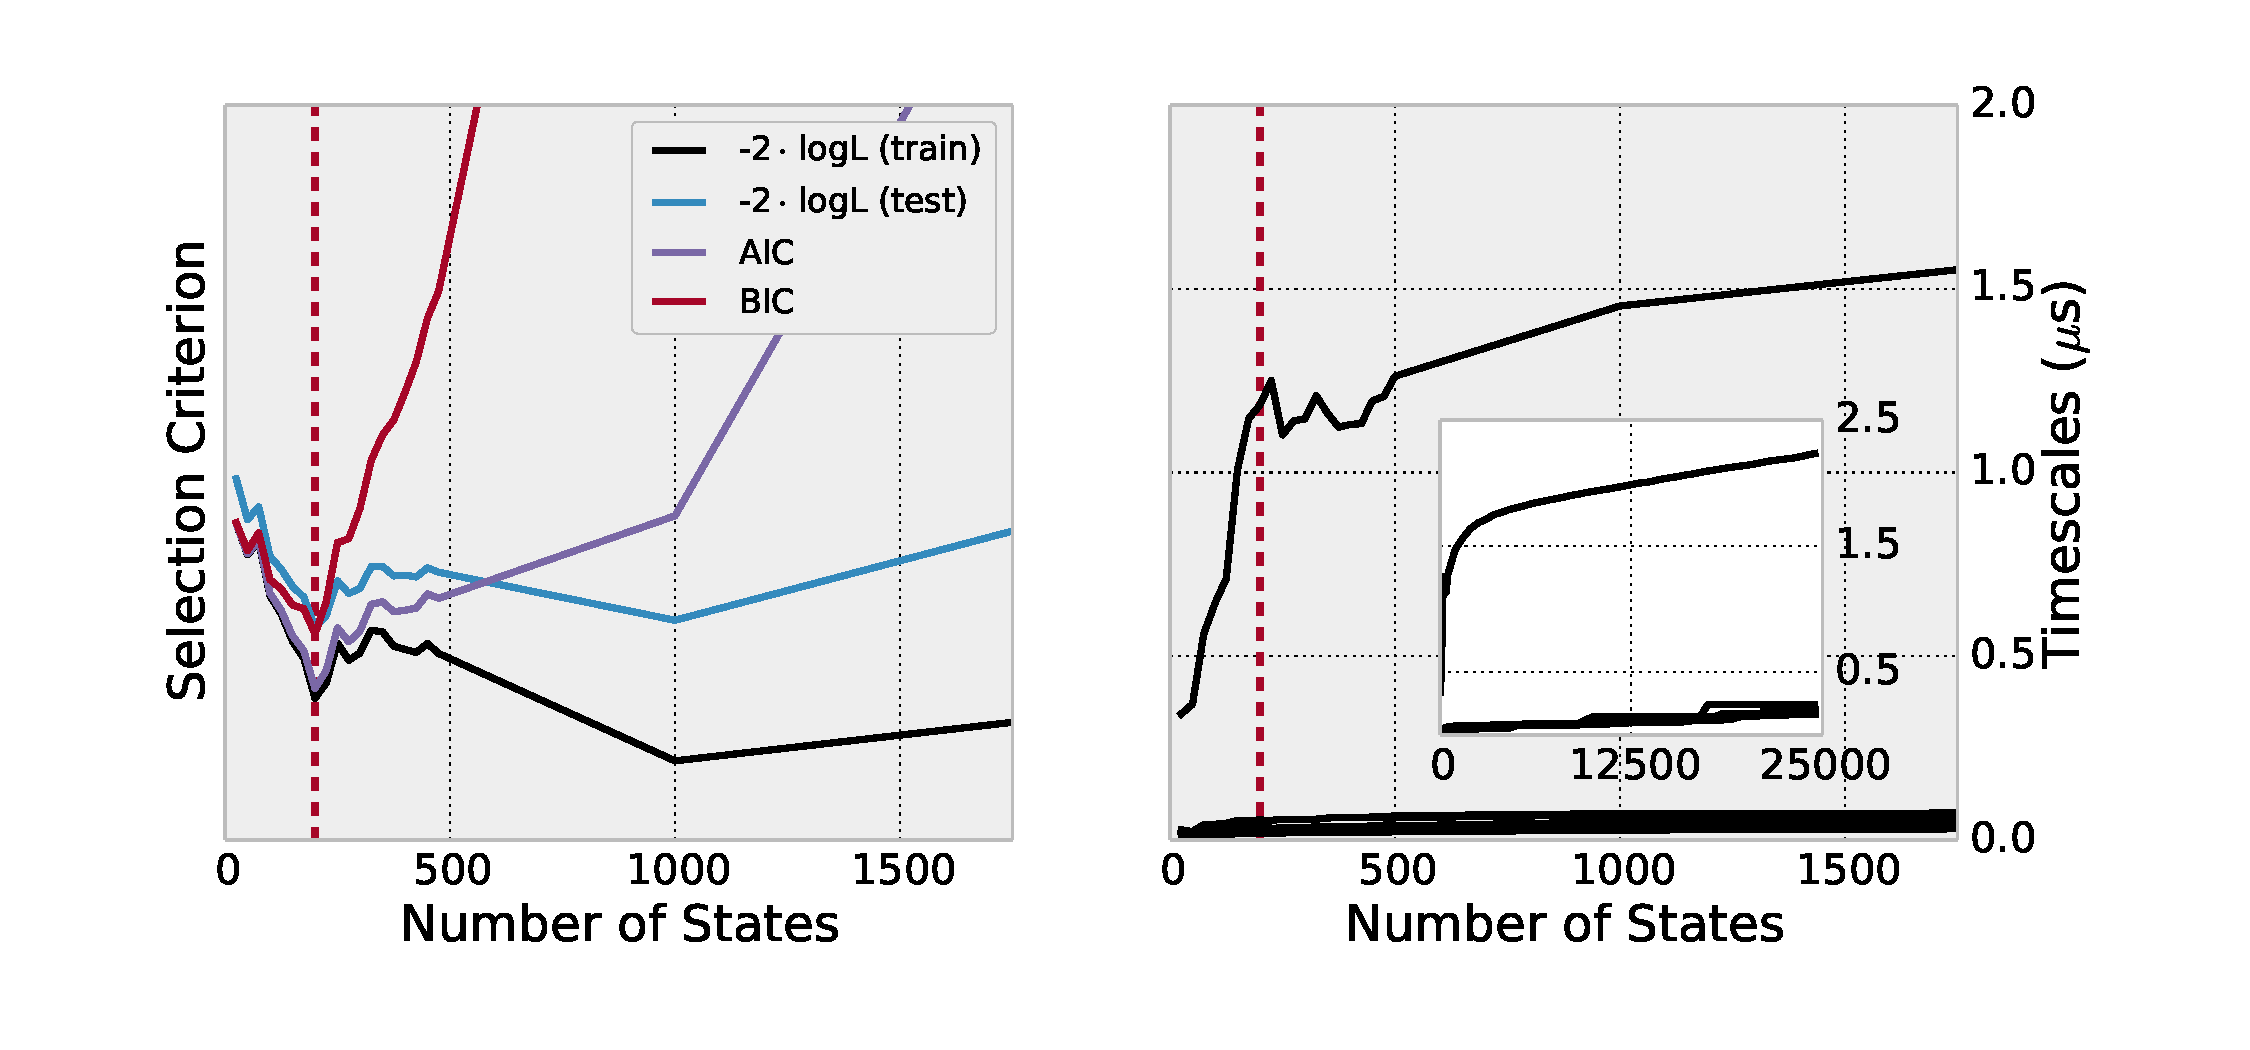
\includegraphics[width=6in]{figs/ww_pca/ww_pca.pdf}
\caption{For MSMs of the WW domain built on the top three PCA components,} 
\end{figure}

%The two 100 $\mu s$ molecular dynamics trajectories of the Fip35 WW domain simulated by \citet{Shaw2010Atomic} have been used to parameterize multiple Markov state models. \citet{Lane2011Markov} proposed a 26,000 state MSM after clustering the data by RMSD, whereas Kellogg et al.,\cite{Kellogg2012Evaluation} clustering on contact maps or secondary structure, proposed 100 and 175 state models, respectively. Consistent with this spread, we find the optimal number of states to be highly dependent on the space in which the data is clustered. With RMSD, the Gaussian likelihood indicates that Markov models built with on the order of 5,000 states optimally balance model quality and generalization error. On the other hand, the tICA method's identification of slow order parameters in the simulations has the effect of reducing the number of states necessary when constructing Markov models. While only using 200-600 states, Markov models constructed using tICA were still able to recapitulate the folding timescale as well as the faster processes identified by McGibbon and Pande\cite{McGibbon2013Learning}.

\subsection{Limitations and Future Work}

The likelihood functions described herein permit the comparison of Markov state models with varying number of states, however, they require that the compared models have the same support. As such, a direct comparison of the likelihoods between models built with tICA and models built with RMSD is not possible. Furthermore, the uniform emission model is intractable for all but the simplest systems. The Gaussian emission model does not have this limitation.

In the future, we plan to extend this work to the consideration of models without discrete states, where the requirement that states strictly partition phase space into a set of discrete indicator functions is relaxed and the models are parameterized by a direct optimization of \cref{eq:like}. This strategy would complement approaches that generalize MSMs beyond discrete states\cite{Noe2013Variational}.

\section{Conclusions}

Markov State Models are powerful and popular frameworks for the analysis of molecular simulations, with a growing literature and two open source software tools\cite{Beauchamp2011Msmbuilder2, Senne2012EMMA}. There are, however a number of steps in the construction process that require hand-tuning, which limits the use of MSMs to experts and introduces significant biases into the model building process. Additionally, the ability to automatically construct MSMs on the fly while simulations are in progress, an important point for so-called adaptive sampling procedures\cite{Bowman2010Enhanced}, is hampered when manual model selection is required. 

These results take a step toward fully automating the MSM construction process and controlling the complexity and generalization error by providing a quantitative method for selecting the most suitably complex model, given the data.

\begin{acknowledgement}
It is an honor and a pleasure to contribute this paper to the Swope Festschrift.  I (V.S.P.) have been working with Bill since my early days at Stanford and have benefitted greatly from our numerous interactions with him.  Bill's insight, clarity of thought, and careful approach has influenced my lab's work very broadly.  I am very pleased that our collaborations continue through today and look forward to many more in the future.
\end{acknowledgement}

\bibliography{bibliography}

\section{Appendix}
\subsection{Other emission distributions}

A more tractable alternative to the uniform distribution is a Gaussian emission model where $P(\mathbf{x} | s(\mathbf{x}))$ is modeled as multivariate normal \cref{eq:like_mvn}.
\begin{equation}
\label{eq:like_mvn}
\begin{split}
P(\mathbf{x}_t | s(\mathbf{x}_t)) = \Bigg[ \frac{1}{(2 \pi)^\frac{d}{2} |\Sigma_{s(\mathbf{x}_t)}|^\frac{1}{2}} \\
   \exp\left(-\frac{1}{2} (\mathbf{x}_t - \bm{\mu}_{s(\mathbf{x}_t)})^T \Sigma_{s(\mathbf{x}_t)}^{-1} (\mathbf{x}_t - \bm{\mu}_{s(\mathbf{x}_t)})\right)\Bigg] 
\end{split}
\end{equation} where $\bm{\mu}_{s(\mathbf{x}_t)}$ is the cluster center assigned to $\mathbf{x}_t$ and $\Sigma_{s(\mathbf{x}_t)}$ is the corresponding covariance matrix. For simplicity, we follow \citet{Pelleg2000Xmeans} and employ a spherical Gaussian model with a single shared variance parameter across the states estimated by maximum likelihood, under which it reduces to:
\begin{equation}
\label{eq:like_mvn2}
 P(\mathbf{x}_t | s(\mathbf{x}_t)) = \frac{1}{\left(2 \pi \hat{\sigma}^2\right)^{\frac{d}{2}}} \exp\left(-\frac{||\mathbf{x}_t - \bm{\mu}_{s(\mathbf{x}_t)}||^2}{2 \hat{\sigma}^2} \right)
\end{equation} where
\begin{equation}
\label{eq:mle_sigma}
\hat{\sigma}^2 = \frac{1}{N - k} \sum_{t=1}^N || \mathbf{x}_t - \bm{\mu}_{s(\mathbf{x}_t)} ||^2
\end{equation} and $k$ is the number of states.

Since the likelihood requires the emission distributions to have zero overlap -- such that each conformation only has nonzero emission probability from a single state, the nonzero overlap between the Gaussian emission distributions introduces a truncation error. One approach to ameliorate this issue is to truncate the density functions at the state boundaries, and renormalize. We assume that the overlaps are small, and use the density defined in \cref{eq:like_mvn2}. An alternative approach for relaxing this approximation is possible with the forward-backward algorithm,\cite{Rabiner1989Tutorial} but is beyond the scope of this work.

We tested the Gaussian likelihood on MSMs built using k-means clustering on the M\"uller potential. The training and test set log-likelihoods, BIC, and AIC are all optimized by a five state model (\cref{fig:kmeans_mull}). The decrease in the training set log-likelihood can be explained by a trade-off inherent in \cref{eq:like}, where adding more states leads to an increase in the emission distribution term but causes the transition matrix term to decrease significantly more. This trade-off illustrates a deficiency in the step-wise approach in which neither the transition matrix nor the state space is parameterized to explicitly optimize the full \cref{eq:like}.

\begin{figure}
\centering
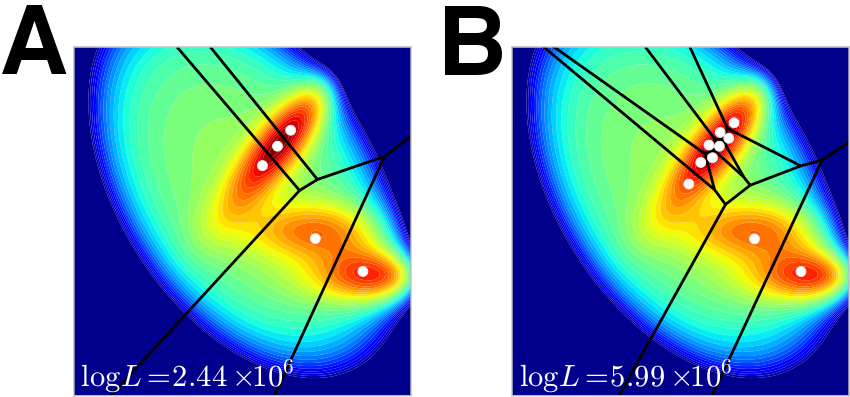
\includegraphics[width=3in]{figs_final/kmeans_like2_lbl.png}
\caption{MSMs were built using k-means clustering on the M\"uller potential simulations. Since k-means optimizes an objective function that is related to the emission probability, our likelihood picks only a few states as the most likely model. The likelihood decreases as new states are introduced, due to a competition between the transition matrix term and emission distribution term in \cref{eq:like}.\label{fig:kmeans_mull}}
\end{figure}

We also tested the Gaussian likelihood on the same WW simulations as discussed above. The complexity of evaluating the Gaussian emission model likelihood does not increase with respect to dimension. Thus we used the Gaussian emission model with both the four-dimensional tICA models and those built using k-centers clustering with the minimal cartesian root-mean squared deviation (RMSD) over Fip35's 252 non-redundant heavy atoms, computed using the quaternion characteristic polynomial method\cite{Theobald2005Rapid}. For evaluating the Gaussian emission likelihood, we used a value of $3 \cdot 252 - 6 = 750$ for the dimension of the emission distribution.


\end{document}


In the finite-data regime, additional complexity in the Markov model, in the form of increasing number of states, does come at a statistical cost.
\begin{itemize}
\item Is the 26,000 state model ``overfit''? The obvious answer, based on the line of reasoning that this paper is taking, is yes. But I think we need to consider the question a little more subtly. Perhaps it depends on what questions we ask of the model. When you ask both a ``properly-fit'' model and an overfit model a question that basically falls within the training set -- and neither of them need to extrapolate or really infer out-of-sample information, they'll both do fine. Heck, the overfit model might do better at telling you exactly what was \emph{in} the data set.
\item The folding timescale is relatively insensitive to differences in MSM construction methodology. This has been observed in many data sets (McGibbon 2013, others). We hypothesize that this behavior is due to the large structural deviations at play -- even a two state model, given the same data-set, could basically get the right timescale just from counting the number of transitions. But finding these other timescales that are structurally subtle is different challenge. Also, how robust are other properties like experimental projections or the MFPT distribution to the number of states?
\item Single trajectory data-sets are ``easier'' for MSMs. One of the uses of MSMs is to ``stitch together'' multiple trajectories -- this function only happens when the states are large enough that they \emph{connect} trajectories, so you can't have too many states in this case. But when you have a single trajectory, there's no possible way to create a disconnected model anyways.
\item We need to state, elegantly if possible, the differences between our likelihood and Liz Kellogg's. This requires some careful language, since we think there are methodological problems with her approach.
\end{itemize}




\begin{itemize}
\item This model doesn't help us pick the lag time.
\item It also doesn't help us pick the projected vector space, at least in a quantitative way. This is kind of a big deal, but it is what it is.
\item Uniform distributions are extremely inconvenient to work with. In the future, we plan to extend this work to Markov state models without discrete states.
\item \{I want to get this in print.\} Going forward, we anticipate that a combination of kinetic dimensionality reduction and clustering is going to be the key combination for robust Markov state model construction. The two approaches are characterized by complementary approximations and sources of error. In dimensionality reduction, the assumption is that the dynamics ``align'' with the vectors in some sense -- we talk about dynamics in the ``x direction'' as having some characteristic, regardless of whether they occur around $x=x_a$ or $x=x_b$. In clustering, if $x_a$ and $x_b$ are in different states, there's no crosstalk at all. A euclidean distance metric is invariant with respect to unitary transforms anyways. But clustering gets ``thrown off'' when you have kinetically irrelevant directions: to get the same resolution with the clusters in the kinetically \emph{relevant} directions, you need a number of states that is exponential in the number of included kinetically \emph{irrelevant} directions. Because the sources of error are complementary, the combination should be uniquely powerful.
\end{itemize}


\begin{itemize}
    \item MSMs are great
    \item They have weaknesses. We are solving them.
    \item The automated selection of the number of states is a critical part of procedures that build MSMs as part of a simulation protocol to drive adaptive sampling. If MD algorithms required user input every couple picoseconds, people would never get anything done.
\end{itemize}



% old stuff about using uniform distributions
However, models' long timescale behavior -- the rates and fluxes between metastable basins -- are independent of the choice of the emission distributions. The emission distributions characterize only the fine details of the equilibrium distribution within states, a quantity that the MSM approach does not seek to model; implicit in the decision to group conformations together into states is the idea that we decline to model the differences between conformations belonging to the same state. If such differences exist and are sufficiently large to warrant attention, than the states are too large.

Therefore, the most appropriate emission distribution for discrete state MSMs is that of the uniform distribution over the phase-space volume of the state. That is, the likelihood of observing a conformation in phase space given that the conformation is assigned to state $i$ is $0$ if the conformation is outside of the bounding volume of the state and constant if the conformation is within the volume. This constant is set so that the distribution integrates to $1$, and is thus the reciprocal volume of the state.


%\begin{figure}
%\centering
%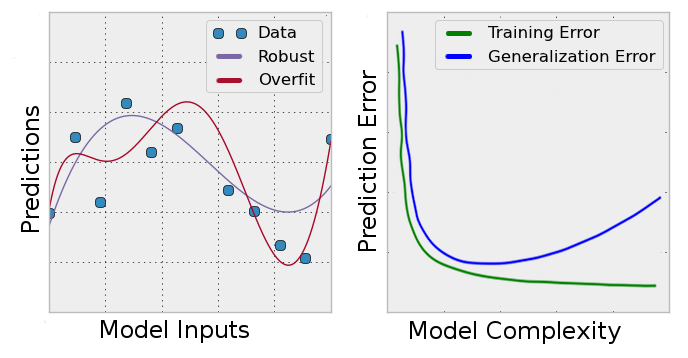
\includegraphics[width=3.1in]{figs/overfitting.png}
%\caption{An example of overfitting. Left: in the presence of noise, a more complex model is able to fit the observed training data better, with lower residues and a higher empirical likelihood, %but fails to distinguish the signal from the noise. Right: more complex model classes exhibit lower training errors, but generalize poorly to unobserved data.}
%\end{figure}




